\chapter{Перехідна функція антени з круговою апертурою}
\label{ch:linear}

%%%%%%%%%%%%%%%%%%%%%%%%%%%%%%%%%%%%%%%%%%%%%%%%%%%%%%%%%%%%%%%%%%%%%%%%%%%%%%%
\section{Наближення кругової апертури}

На початку 70х років інтерес до імпульсної радіофізики був збуджений
мілітарним застосуванням переваг нанширокосмугових радарних та 
телекомунікаційних систем, як в Україні \cite{imp:Dumin1996} так 
і за кордоном \cite{imp:BaumIN0105}. Соьгодні, наробітки минулого 
століття знайшли своє застосування у системах інтернету речей, як 
наприклад Apple SoC U1 % \cite{}.

Широким класом технічних рішень для напрямленого випромінювання 
надширокосмугового електричного струму є антени імпульсного віпромінювання.
Серех них можна виділити чотири класи за способом вирівнювання фронту хвиль:
%
\begin{enumerate}
	\item Без вирівнювання сферичного фронту
	\item Лінзеві сповільнювачі
	\item Рефлекторні антени
	\item Комбіновані архітектури \cite{imp:BaumSSN0379}
\end{enumerate}

Живлення такого класу антен зазвичай виконується ТЕМ рупором, що підєднується 
до коаксіального кабеля через балун. Кожен з перелічиних типів антен має свої
переваги, недоліки та сферу застосування. Даний розділ присвячуєтся 
дослідженню саме лінзевих антен імпульсного випрмінювання (LIRA). 

Антени типу LIRA мають численні переваги над рефлекторними. Перш за все це
більш високий ковіціент підсилення антенни \cite{imp:BaumUWBSP1}. Подруге,
лінзеві антени не мають області тіні від опромінювача та краще узгоджуються
на практиці \cite{imp:BaumSSN0377}. Також експерементальне порівняння LIRA 
та RIRA показують меншої тривалості. З недоліків варто відзначити важкість 
виготовлення лінз точної форми та вагу антени.

Розглянемо задачу збудження такої антени нестаціонарним імпульсним струмом,
деякої часової залежності $ f(t) $, з умовою існування першої та другої 
похідної. Ефективна тривалісь перехідного процессу $ f(t) $ за метрикою FWHM 
розглядається в межах від десятків піко-секунд до декількох нано-секунд.

Сферична хвиля проходе через систему діелектричних лінз розташованих у 
розкриві формуючи квазі-одномоментне збудження плаского фронту у розкриві. 
Формою розкриву зазвичай вибирають кругову апертуру. Таким чином, у першому 
наближенні, у розкриві формується рівномірно розподілений сторонній плаский 
електричний струм напрямлений від одного плеча рупора до іншого. Вперше така
апроксимація була запропонована 1985р. \cite{imp:Wu1985} та 
емпірично перепірена 1991р. \cite{imp:Wu1991}.

Серед лінзевого класу антен, що формують розподіл сторонього струму у вигяди 
плаского диску варто відзачити антену Рис.~\ref{fig:lira_baum}, що спершу
представив Ву \cite{imp:Wu1987}, а згодом і Баум \cite{imp:BaumSSN0377}. 
Лінза антени виконана у формі витягнутого сфероїда, а розкрив ТЕМ рупора 
цілком заповнено діелектриком. Таким чином мінімалізується відбиття. 
Зкруглений рупор починається в одному фокусі еліпсоїда, а закінціється в 
другому, таким чином радіус розкриву є факальним параметром еліпсоїда.
В якості матеріалу для лінзи пропонується використовувати поліетилен 
високої густини ($\epsilon = 2.3 $).

\begin{figure}[htbp] \begin{center}
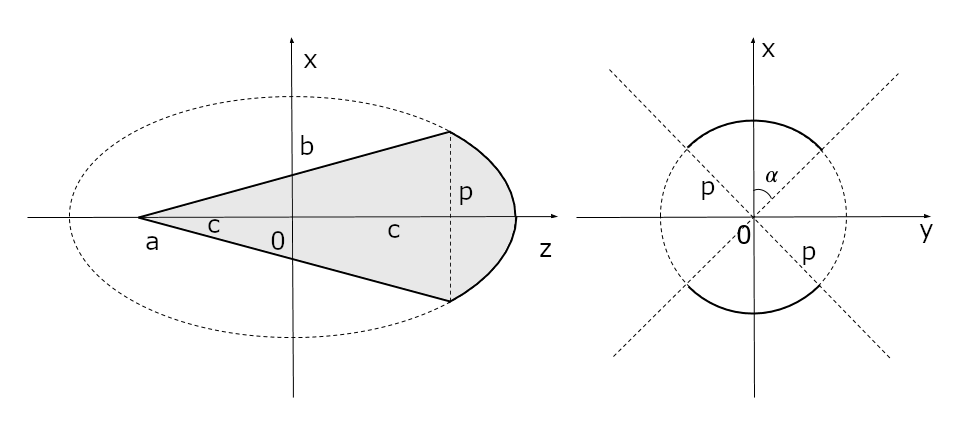
\includegraphics[scale=0.5]{Baum_LIRA}
\caption{Геометрія лінзевої антени Баума та Ву} \label{fig:lira_baum}
\end{center} \end{figure}

В 1991р. Ву представив антену, що краще підходить під наближення  
плаского диску електричного струму \cite{imp:Wu1991}. Гіперболічна лінза 
забеспечує розташування площини рівних фаз в самому розкриві, що і утворює
плаский диск \ref{fig:lira_wu}. Цікавою варіацією цієї антени є заміна 
діелектричного наповнення $ \epsilon_1 $ та лінзи $ \epsilon_2 $ на матрвал,
діелектрична характеристика якого є функцією координат $ \epsilon(\rho, z) $.
Таким чином відбиття від внутрішньої поверхні лінзи зникне і характиристики 
антени покращаться. Важливим мінусом такої архітектуре стає важкість 
виготовлення лінзи.

\begin{figure}[htbp] \begin{center}
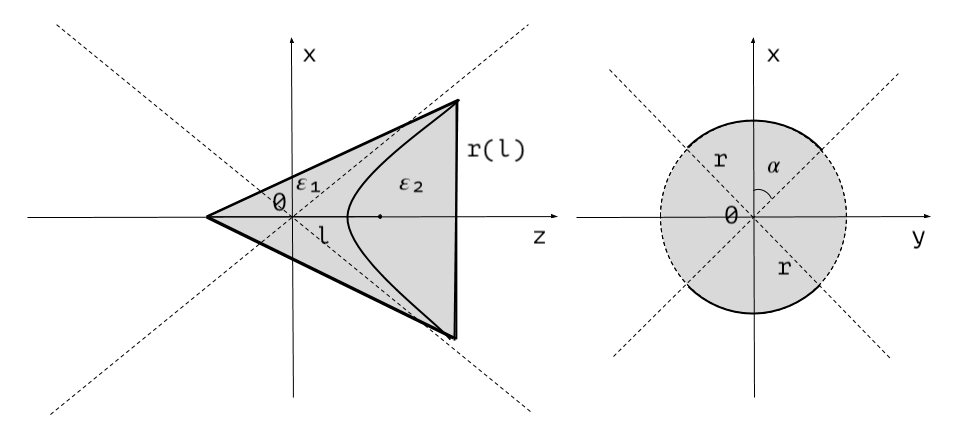
\includegraphics[scale=0.5]{Wu_LIRA}
\caption{Геометрія лінзевої антени Ву} \label{fig:lira_wu}
\end{center} \end{figure}

Прямим призначенням таких антен є телекомунікація, радіолокація і лабораторні 
вимірювання. Проте цікавість таких антен пояснюється ще і аномально повільним
згасанням енергії імпульсного поля з відстанню, що було теоретично 
передбачено \cite{imp:Wu1987}. Цей ефект відомий за назвою електромагнітний 
сняряд.

Фізична модель плаского диску описує поле LIRA лише у першому наближенні.
Така модель не враховує вихровий магнітний сторонній струм, що існує на ряду 
з пласким електричним, а також не враховує струми що течуть назад в генератор 
відбившись від краю рупора - поле такого струму залишає довгий "хвіст" після 
основного імпульу. Проте емпіричне дослідженнях 
\cite{imp:BaumSSN0396,imp:BaumSSN0401} показує, що при належному 
узгодженні, паразитний вплив відбиття фактично відсутній, а перехідна 
функція отримана експерементальним шляхом відповідає розвязку, що дає 
плаский диск.

Розв'язок задачі плаского диску шукали разними методами. Першими були 
отримані наближені розв'язки в частотній області 
\cite{imp:Wu1985,imp:Sodin1992-10}. Також, розвязок для цієї задачі знайдено 
у часовій області \cite{imp:Dumin1996}. Недоліком наявних розвязків є те,
що вони не надають часову залежніть напруженності поля в довільних точках 
спостереження в явному виді. При самодії поля крізь середовище на значення 
напруженності поля в кожній точці спостереження та в будь-який момент впливать
всі пов'язані зі спостереженням події. Таким чином наявність розв'язання в 
будьякій точці спостереження - необхідна умова.
%
%%%%%%%%%%%%%%%%%%%%%%%%%%%%%%%%%%%%%%%%%%%%%%%%%%%%%%%%%%%%%%%%%%%%%%%%%%%%%%%
\section{Розв'язання методом еволюційних рівнянь}
%
Розглянемо сторонній електричний нестаціонарний струм $ \vect{j_0} (r,t) $ 
в якості единого джерела електромагнітнго поля. Нехай, струм однонапрямлений, 
рівномірнорозподілений та має форму плаского диску нульової товщини. Для 
розв'язання прямої задачі електродинаміки для довільної часової $ f(t) $ 
залежності нестаціонарного струму $ \vect{j_0} (r,t) $, достатньо отримати
розв'язок для перехідної функції, тобто $ f(t) = H(t) $, де $ H(t) $ - 
функція Хевісайда. Тоді, математично його можна описати в циліндричних
координатах $ \rho, \varphi, z $, як
%
\begin{equation}
\vect{j_0} \left( r, t \right) = \vect{J} = \vect{x_0} A_0 H(t) \delta(z) 
\left(  H(\rho) - H(\rho - R) \right),
\end{equation}
%
де $ A_0 $ - максимальна амплітуда струму, $ R $ - радіус диску,
$ \delta(z) $ - символ Кронекера, а 
$ \vect{x_0} = \vect{\rho_0} \cos \varphi - \vect{\varphi_0} \sin \varphi $ 
- декартовий орт OX. 
%
\begin{figure}[htbp] \begin{center}
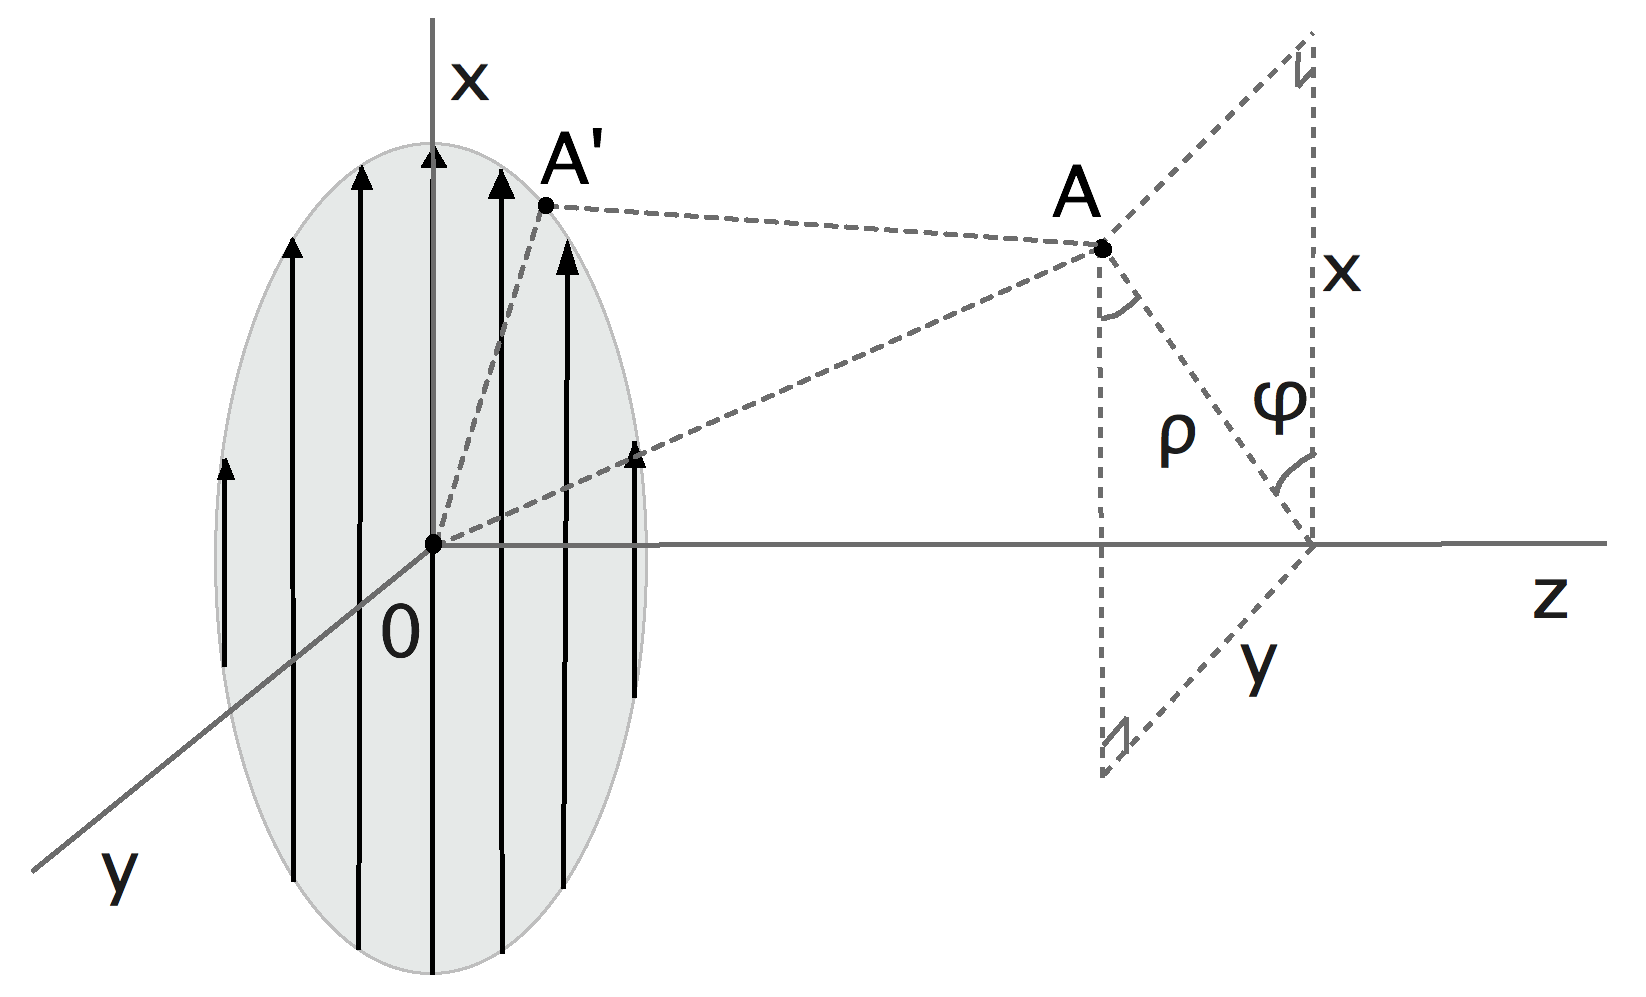
\includegraphics[scale=0.55]{PlaneDisk}
\caption{Геометрія випромінювача} \label{fig:pdisk}
\end{center} \end{figure}
%
\textcolor{lightgray} { \begin{equation*} \begin{aligned}
\begin{cases}
\vect{\rho_0} = \vect{x_0} \cos \varphi + \vect{y_0} \sin \varphi \\
\vect{\varphi_0} = - \vect{x_0} \sin \varphi + \vect{y_0} \cos \varphi
\end{cases} \Rightarrow \mathbf{A} = \left( \begin{array}{cc}
\cos \varphi & \sin \varphi \\
- \sin \varphi & \cos \varphi
\end{array} \right)
\end{aligned} \end{equation*} }
%
\textcolor{lightgray} { \begin{equation*} \begin{aligned}
\vect{j_0} \left( \vect{\rho_0}, \vect{\varphi_0} \right) = 
\mathbf{A} \vect{j_0} \left( \vect{x_0}, \vect{y_0} \right) = \\
= H(t) \delta(z) (  H(\rho) - H(\rho - R) ) 
( \vect{\rho_0} \cos \varphi - \vect{\varphi_0} \sin \varphi )
\end{aligned} \end{equation*} }
%
Для застосування методу еволюційних рівнянь знайдемо модовий розклад 
струму
%
\begin{equation} \label{eq:jm_base}
j_m \left( r, t; \nu \right) = \frac{\sqrt{\mu_0}}{2\pi} 
\int \limits_{0}^{2\pi} d \varphi \int \limits_{0}^{\infty} \rho d \rho 
\vect{j_0} \crossprod{ \nabla_\perp \Psi_m^* }{ \vect{z_0} },
\end{equation}
%
де $ \Psi_m^* $ - комплексно спряжена бізисна функція \cite{imp:Dumin2010}.
%
\textcolor{lightgray} { \begin{equation*} \begin{aligned}
\crossprod{ \nabla_\perp \Psi_m^* }{ \vect{z_0} } = 
- \sqrt{\nu} e^{-im\varphi} \left( 
\vect{\varphi_0} \frac{J_{m-1} (\nu \rho) - J_{m+1} (\nu \rho)}{2} + 
\right. \\ + \left. i m \vect{\rho_0} \frac{J_m (\nu \rho)}
{\rho \nu} \right) = - \sqrt{\nu} e^{-im\varphi} \left( 
\vect{\varphi_0} \frac{J_{m-1} (\nu \rho) - J_{m+1} (\nu \rho)}{2} + 
\right. \\ + \left. i \vect{\rho_0} \frac{J_{m-1} (\nu \rho) + 
J_{m+1} (\nu \rho)}{2} \right)
\end{aligned} \end{equation*} }
%
\textcolor{lightgray} { \begin{equation*} \begin{aligned}
\vect{j_0} \crossprod{ \nabla_\perp \Psi_m^* }{ \vect{z_0} } = 
- \sqrt{\nu} ( \cos m \varphi - i \sin m \varphi ) 
H(t) \delta(z) ( H(\rho) - H(\rho - R) ) \cdot \\ \cdot \left( 
i \frac{J_{m-1} (\nu \rho) + J_{m+1} (\nu \rho)}{2} \cos \varphi
- \frac{J_{m-1} (\nu \rho) - J_{m+1} (\nu \rho)}{2} \sin \varphi
\right)
\end{aligned} \end{equation*} }
%
\textcolor{lightgray} { \begin{equation*} \begin{aligned}
j_m = \frac{\sqrt{\mu_0}}{2\pi} \sqrt{\nu} \delta(z) H(t) \cdot \\
\cdot \Big( \int \limits_{0}^{2\pi} d \varphi \sin \varphi 
( \cos m \varphi - i \sin m \varphi) \int \limits_{0}^{R} 
\frac{J_{m-1} (\nu \rho) - J_{m+1} (\nu \rho)}{2} \rho d \rho - \\
- i \int \limits_{0}^{2\pi} d \varphi \cos \varphi 
( \cos m \varphi - i \sin m \varphi) \int \limits_{0}^{R} 
\frac{J_{m-1} (\nu \rho) + J_{m+1} (\nu \rho)}{2} \rho d \rho \Big)
\end{aligned} \end{equation*} }
%
\textcolor{lightgray} { \begin{equation*} \begin{aligned}
j_m = \frac{\sqrt{\mu_0}}{2\pi} \sqrt{\nu} \delta(z) H(t) 
i\pi ( \delta_{m,-1} - \delta_{m,1} ) \int \limits_{0}^{R} 
\frac{J_{m-1} (\nu \rho) - J_{m+1} (\nu \rho)}{2} \rho d \rho - \\
- \frac{\sqrt{\mu_0}}{2\pi} \sqrt{\nu} \delta(z) H(t) 
i\pi ( \delta_{m,-1} + \delta_{m,1} ) \int \limits_{0}^{R} 
\frac{J_{m-1} (\nu \rho) + J_{m+1} (\nu \rho)}{2} \rho d \rho =
\end{aligned} \end{equation*} }
%
\textcolor{lightgray} { \begin{equation*} \begin{aligned}
= i \frac{\sqrt{\mu_0 \nu}}{4} \delta(z) H(t)
\delta_{m,-1} \int \limits_{0}^{R} \left( J_{-2} (\nu \rho) - 
J_0 (\nu \rho) \right) \rho d \rho - \\
- i \frac{\sqrt{\mu_0 \nu}}{4} \delta(z) H(t)
\delta_{m,1} \int \limits_{0}^{R} \left( J_{0} (\nu \rho) - 
J_2 (\nu \rho) \right) \rho d \rho - \\
- i \frac{\sqrt{\mu_0 \nu}}{4} \delta(z) H(t)
\delta_{m,-1} \int \limits_{0}^{R} \left( J_{-2} (\nu \rho) +  
J_0 (\nu \rho) \right) \rho d \rho - \\
- i \frac{\sqrt{\mu_0 \nu}}{4} \delta(z) H(t)
\delta_{m,1} \int \limits_{0}^{R} \left( J_{0} (\nu \rho) +
J_2 (\nu \rho) \right) \rho d \rho =
\end{aligned} \end{equation*} }
%
\textcolor{lightgray} { \begin{equation*} \begin{aligned}
= - i \frac{\sqrt{\mu_0 \nu}}{2} \delta(z) H(t) 
(\delta_{m,1} + \delta_{m,-1}) 
\int \limits_{0}^{R} \left( J_{0} (\nu \rho) + 
J_2 (\nu \rho) \right) \rho d \rho - \\
- i \frac{\sqrt{\mu_0 \nu}}{2} \delta(z) H(t) 
(\delta_{m,1} + \delta_{m,-1}) 
\int \limits_{0}^{R} \left( J_{0} (\nu \rho) -
J_2 (\nu \rho) \right) \rho d \rho = \\
= - i \frac{\sqrt{\mu_0 \nu}}{2} \delta(z) H(t) 
(\delta_{m,1} + \delta_{m,-1}) 
\int \limits_{0}^{R} J_{0} (\nu \rho) \rho d \rho
\end{aligned} \end{equation*} }
%
\textcolor{lightgray} { \begin{equation*} \begin{aligned}
\int \limits_{0}^{R} J_{0} (\nu \rho) \rho d \rho = 
\frac{1}{\nu^2} \int \limits_{0}^{R} J_{0} (\nu \rho) \nu \rho d \nu \rho =
\left. \frac{\rho J_1 (\nu \rho) }{\nu} \right|_{0}^{R} = 
\frac{R J_1 (\nu R)}{\nu}
\end{aligned} \end{equation*} }
%
Після інтегрування $ \eqref{eq:jm_base} $ отримаємо тільки дві не нульові 
рівнімоди, визначені через симполи кронекера $ \delta_{m,\pm1} $.
%
\begin{equation} 
j_m (z, t; \nu) = - i R A_0 \frac{\sqrt{\mu_0}}{2} \delta(z) H(t) 
\frac{\delta_{m,1} + \delta_{m,-1}}{\sqrt{\nu}} J_1 (\nu R)
\end{equation}
%
Тепер знайдемо продольні модові коефіцієнти $ h_1 $ та $ h_{-1} $ розв'язанням 
рівняннь Клейна-Гордона
%
\textcolor{lightgray} { \begin{equation*} \begin{aligned}
- \epsilon \partial_{ct} (V_m^h) - \partial_z I_m^h + \nu^2 h_m = 
\frac{\sqrt{\mu_0}}{2 \pi} \int_0^{2\pi} d \varphi 
\int_0^{\infty} \rho d \rho \crossprod{\vect{z_0}}{\vect{J_\perp}}
\nabla_\perp \Psi_m^* (\nu) 
\end{aligned} \end{equation*} }
%
\textcolor{lightgray} { \begin{equation*} \begin{aligned}
\crossprod{\vect{z_0}}{\vect{J_\perp}} \nabla_\perp \Psi_m^* (\nu) =
\vect{J_\perp} \crossprod{\nabla_\perp \Psi_m^* (\nu)}{\vect{z_0}}
\end{aligned} \end{equation*} }
%
\textcolor{lightgray} { \begin{equation*} \begin{aligned}
\epsilon \partial_{ct} \left( \mu \partial_{ct} h_m \right) -
\mu^{-1} \partial_z \left( \mu  \partial_z h_m \right) + 
\nu^2 h_m = j_m (z,t,\nu)
\end{aligned} \end{equation*} }
%
\begin{equation} \begin{aligned} \label{eq:klein_gordon}
\frac{\epsilon \mu}{c^2} \frac{\partial^2 h_m}{\partial t^2} - 
\frac{\partial^2 h_m}{\partial z^2} + \nu^2 h_m = j_m (z,t,\nu).
\end{aligned} \end{equation}
%
Рівняння \eqref{eq:klein_gordon} було отримано з припущенням, що середовище 
в якому розповсюджується поле однорідне, стаціонарне та характерезуеться 
видносною діелектричною $ \epsilon $ та магнітною $ \mu $ проникністями.
Буде зречно позначити швидкість світла в цьому середовищі за 
$ \mathit{v} = \frac{c}{\sqrt{\epsilon \mu}} $. Рівняння Клейна-Гордона
має відомий розв'язок через функцію Рімана:
%
\begin{equation} \label{eq:klein_gordon_sol}
h_m (z, t; \nu) = \iint_S j_m (t',z') G(t,t',z,z') dt' dz',
\end{equation}
%
де $ G(t,t',z,z') $ функція Рімана 
%
\begin{equation*}
G = \frac{\mathit{v}}{2} H \left( \mathit{v} (t-t') - (z-z') \right)
J_0 \left( \nu \sqrt{\mathit{v}^2 (t-t')^2 - (z-z')^2} \right).
\end{equation*}
%
З вигляду розв'язоку \eqref{eq:klein_gordon_sol} можна зробити висновок, що
функція Рімана $ G(t,t',z,z') $ - це аналог фунгції Гріна в часовому просторі,
а тобто розв'язок рівняння Клейна-Гордона є еквівалентом принціпу суперпозиції
сферичних нестаціонарних хвиль, що випромінюються кожною з точок джерела у
деякій точці спостереження у визначений час.
%
\textcolor{lightgray} { \begin{equation*} \begin{aligned}
h_m (z, t; \nu) = - i \mathit{V} R \frac{\sqrt{\mu_0}}{4} 
\frac{\delta_{m,1} + \delta_{m,-1}}{\sqrt{\nu}} J_1 (\nu R)
\int \limits_{0}^{\infty} \delta(z) \cdot \\ \cdot
\int \limits_{t - \frac{z}{\mathit{V}}}^{0} 
J_0 \left( \nu \sqrt{\mathit{V}^2 (t-t')^2 - (z-z')^2} \right) dt' dz' = 
i \mathit{V} R \frac{\sqrt{\mu_0}}{4} 
\frac{\delta_{m,1} + \delta_{m,-1}}{\sqrt{\nu}} J_1 (\nu R)
\cdot \\ \cdot \int \limits_{0}^{\infty} \delta(z)
\int \limits_{0}^{t - \frac{z}{\mathit{V}}} 
J_0 \left( \nu \sqrt{\mathit{V}^2 (t-t')^2 - (z-z')^2} \right) dt' dz
\end{aligned} \end{equation*} }
%
\textcolor{lightgray} { \begin{equation*} \begin{aligned}
h_m (z, t; \nu) = i \mathit{V} R \frac{\sqrt{\mu_0}}{4} 
\frac{\delta_{m,1} + \delta_{m,-1}}{\sqrt{\nu}} J_1 (\nu R)
\int \limits_{0}^{t - \frac{z}{\mathit{V}}} 
J_0 \left( \nu \sqrt{\mathit{V}^2 (t-t')^2 - z^2} \right) dt'
\end{aligned} \end{equation*} }
%
Користуючись властивостями дельта-функції Дірака та функції Хевісайда 
запишимо поздовжні модові коефіцієнти $ h_1 $ та $ h_{-1} $ в наступному 
виді:
%
\begin{equation} \label{eq:hm_int}
h_m = \frac{i R A_0}{4} \frac{\delta_{m,1} + \delta_{m,-1}}
{\sqrt{\nu} \sqrt{\epsilon_0 \epsilon \mu}} J_1 (\nu R) 
\int \limits_{0}^{t - \frac{z}{v}} 
J_0 \left( \nu \sqrt{v^2 (t-t')^2 - z^2} \right) dt'
\end{equation} }
%
Зараз зручно перейти до отримання поперечних модових коефіціентів.
Для отримання виразу для $ V_m^h = - \frac{\mu}{c} \partder{h_m}{t} $
необовязково брати інтеграл в $ h_m $ спробуємо спростити вираз 
скориставшись залежністю через похідну по часу, тобто застосуємо 
правило інтерування Лейбніца \cite{imp:Flanders1973}, помітивши, що
%
\begin{equation*} \begin{aligned}
\partder{}{t'} J_0 \left( \nu \sqrt{v^2 (t-t')^2 - z} \right) =
- \partder{}{t} J_0 \left( \nu \sqrt{v^2 (t-t')^2 - z} \right) 
\end{aligned} \end{equation*}
%
отримаємо
%
\textcolor{lightgray} { \begin{equation*} \begin{aligned}
\partder{}{\theta} \int_{a(\theta)}^{b(\theta)} f(x,\theta) dx = 
\int_{a(\theta)}^{b(\theta)} \partder{f}{\theta} dx + 
f\big( b(\theta), \theta \big) \partder{b}{\theta} -
f\big( a(\theta), \theta \big) \partder{a}{\theta}
\end{aligned} \end{equation*} }
%
\textcolor{lightgray} { \begin{equation*} \begin{aligned}
\partder{}{t} J_0 \left( \nu \sqrt{v^2 (t-t')^2 - z} \right) = 
- \nu J_1 \left( \nu \sqrt{v^2 (t-t')^2 - z} \right) 
\partder{}{t} \sqrt{v^2 (t-t')^2 - z} = \\
-  J_1 \left( \nu \sqrt{v^2 (t-t')^2 - z} \right)
\frac{2 \nu v^2 (t-t')}{2 \sqrt{v^2 (t-t')^2 - z}} = - \nu v^2 (t-t') 
\frac{J_1 \left( \nu \sqrt{v^2 (t-t')^2 - z} \right)}
     {\sqrt{v^2 (t-t')^2 - z}}
\end{aligned} \end{equation*} }
%
\textcolor{lightgray} { \begin{equation*} \begin{aligned}
\partder{}{t} \int \limits_{0}^{t - \frac{z}{v}} 
J_0 \left( \nu \sqrt{v^2 (t-t')^2 - z^2} \right) dt' = \\
= \int \limits_{0}^{t - \frac{z}{v}} 
\partder{}{t} J_0 \left( \nu \sqrt{v^2 (t-t')^2 - z^2} \right) dt' +
J_0 (0) - 0 \cdot \left( \nu \sqrt{v^2 (t-t')^2 - z^2} \right) = \\
= - \int \limits_{0}^{t - \frac{z}{v}} 
\partder{}{t'} J_0 \left( \nu \sqrt{v^2 (t-t')^2 - z^2} \right) dt' + 1 =
- \Big. J_0 \left( \nu \sqrt{v^2 (t-t')^2 - z^2} \right) \Big|_{0}^{t - \frac{z}{v}} + 1 = \\
- J_0 \left( \nu \sqrt{z^2 - z^2} \right) + J_0 \left( \nu \sqrt{v^2 t^2 - z^2} \right) + 1 = 
J_0 \left( \nu \sqrt{v^2 t^2 - z^2} \right)
\end{aligned} \end{equation*} }
%
\begin{equation*} \begin{aligned}
\partder{}{t} \int \limits_{0}^{t - \frac{z}{v}} 
J_0 \left( \nu \sqrt{v^2 (t-t')^2 - z^2} \right) dt' =
J_0 \left( \nu \sqrt{v^2 t^2 - z^2} \right),
\end{aligned} \end{equation*}
%
\textcolor{lightgray} { \begin{equation*} \begin{aligned}
V_m^h = - \frac{\mu}{c} \partder{h_m}{t} = 
\sqrt{\mu_0} \sqrt{\frac{\mu}{\epsilon}} \frac{iR A_0}{4} 
\frac{\delta_{m,1} + \delta_{m,-1}}{\sqrt{\nu}} J_1 (\nu R)
J_0 \left( \nu \sqrt{\mathit{v}^2 t^2 - z^2} \right)
\end{aligned} \end{equation*} }
%
тоді можемо записати формулу для коефійієнтів $ V_m^h $
%
\begin{equation} \label{eq:vmh}
V_m^h (z, t; \nu) = - \frac{iR A_0}{4} \sqrt{\frac{\mu_0 \mu}{\epsilon}} 
\frac{\delta_{m,1} + \delta_{m,-1}}{\sqrt{\nu}} J_1 (\nu R)
J_0 \left( \nu \sqrt{\mathit{v}^2 t^2 - z^2} \right).
\end{equation}
%
Далі отримаемо модовий коефіціент $ I_m^h $, що знадобиься для визначення
магнітних компонентів поля. Для цього запишемо поздовжний магнітний модовий
коефіцієнт \cite{eq:hm_int} через спеціальну функцію Ломмеля для двох 
змінних (дійсної та уявної) \cite{imp:Boersma1961}:
%
\textcolor{lightgray} { \begin{equation*} \begin{aligned}
\int \limits_{0}^{t - \frac{z}{\mathit{v}}} 
J_0 \left( \nu \sqrt{\mathit{v}^2 (t-t')^2 - z^2} 
\right) dt' = \left[ \begin{array}{cc} 
\nu \mathit{v} (t-t') = s & t' = t - \frac{ds}{\nu \mathit{v}} \\
dt' = -\frac{ds}{\nu \mathit{v}} & \\
s(0) = \nu \mathit{v} t & s \left( t - \frac{z}{\mathit{v}} \right) = \nu z
\end{array} \right] = \\ = - \frac{1}{\nu \mathit{v}} 
\int_{\nu \mathit{v} t}^{\nu z} ds 
J_0 (\sqrt{s^2 - \nu^2 z^2}) = \frac{1}{\nu \mathit{v}} 
\int_{\nu z}^{\nu \mathit{v} t} ds
J_0 (\sqrt{s^2 - \nu^2 z^2})
\end{aligned} \end{equation*} }
%
\textcolor{lightgray} { \begin{equation*} \begin{aligned}
\int_{\nu z}^{\nu \mathit{v} t} ds e^{-i0s} J_0 (\sqrt{s^2 - \nu^2 z^2}) = \\ 
= \frac{1}{i} (U_1[W_+,Z] + i U_2[W_+,Z] - U_1[W_-,Z] - i U_2[W_-,Z]) = \\
= \frac{1}{i} (-U_1[W_-,Z] + i U_2[W_+,Z] - U_1[W_-,Z] - i U_2[W_+,Z]) = \\
= \left[ \begin{array}{c} W_\pm = \pm i (\nu \mathit{v} t - \nu z) \\
Z = \sqrt{\nu^2 \mathit{v}^2 t^2 - \nu^2 z^2} \end{array} \right] = 
2i U_1 \left[ -i \nu (\mathit{v}t-z), \nu \sqrt{\mathit{v}^2 t^2-z^2} \right]
\end{aligned} \end{equation*} }
%
\textcolor{lightgray} { \begin{equation*} \begin{aligned}
\int \limits_{0}^{t - \frac{z}{\mathit{v}}} 
J_0 \left( \nu \sqrt{\mathit{v}^2 (t-t')^2 - z^2} 
\right) dt' = \frac{2i}{\nu \mathit{v}} U_1 
\left[ -i \nu (\mathit{v}t-z), \nu \sqrt{\mathit{v}^2t^2-z^2} \right]
\end{aligned} \end{equation*} }
%
\textcolor{lightgray} { \begin{equation*} \begin{aligned}
h_m (z, t; \nu) = \mathit{v} \sqrt{\mu_0} \frac{iR A_0}{4} 
\frac{\delta_{m,1} + \delta_{m,-1}} {\sqrt{\nu}} J_1 (\nu R) 
\frac{2i}{\nu \mathit{v}} U_1 \left[ W_-, Z \right]
\end{aligned} \end{equation*} }
%
\begin{equation} \label{eq:hm_lommel}
h_m (z, t; \nu) = - \sqrt{\mu_0} \frac{R A_0}{2} 
\frac{\delta_{m,1} + \delta_{m,-1}}
{\nu^{3/2}} J_1 (\nu R) U_1 \left[ W_-, Z \right]
\end{equation}
%
Тепер підставивши \eqref{eq:hm_lommel} в вираз для коефіціенту
$ I_{m}^{h} = \partder{h_m}{z} $ отримаємо:
%
\textcolor{lightgray} { \begin{equation*} \begin{aligned}
I_{m}^{h} = \partder{h_m}{z} = 
- \sqrt{\mu_0} \frac{R A_0}{2} 
\frac{\delta_{m,1} + \delta_{m,-1}}
{\nu^{3/2}} J_1 (\nu R) \partder{}{z} U_1 [ W_-, Z ]
\end{aligned} \end{equation*} }
%
\textcolor{lightgray} { \begin{equation*} \begin{aligned}
\begin{array}{lcr}
\derivat{W_-}{z} = i \nu & &
\derivat{Z}{z} = \frac{\nu}{2 \sqrt{\mathit{V}^2 t^2 - z^2}} (-2z) = 
- \frac{\nu z}{\sqrt{\mathit{V}^2 t^2 - z^2}} \\
\end{array}
\end{aligned} \end{equation*} }
%
\textcolor{lightgray} { \begin{equation*} \begin{aligned}
\left( \frac{Z}{W} \right)^2 = 
\left( - \frac{ \sqrt{\mathit{V}^2 t^2-z^2}}{i(\mathit{V} t-z)} \right)^2 =
\left( \frac{ i \sqrt{\mathit{V}^2 t^2-z^2}}{\mathit{V}t-z} \right)^2 =
- \frac{\mathit{V}^2 t^2-z^2}{(\mathit{V} t-z)^2} = 
- \frac{\mathit{V}t+z}{\mathit{V}t-z}
\end{aligned} \end{equation*} }
%
\textcolor{lightgray} { \begin{equation*} 
\partder{}{Z} U_n (W,Z) = - \frac{Z}{W} U_{n+1} (W,Z)
\end{equation*} }
%
\textcolor{lightgray} { \begin{equation*}
2 \partder{}{W} U_n (W,Z) = U_{n-1} (W,Z) + 
\left( \frac{Z}{W} \right)^2 U_{n+1} (W,Z)
\end{equation*} }
%
\textcolor{lightgray} { \begin{equation*} \begin{aligned}
\partder{}{z} U_1 \left[ -i \nu (ct-z), \nu \sqrt{c^2t^2-z^2} \right] =
\partder{}{z} U_1[W,Z] = \partder{U_1}{W} \derivat{W}{z} + 
\partder{U_1}{Z} \derivat{Z}{z} = \\
= \frac{i \nu}{2} \left( U_0 - \frac{ct+z}{ct-z} U_2 \right) -
\frac{\nu z}{\sqrt{c^2t^2 - z^2}} 
\left( - \frac{i \sqrt{c^2t^2-z^2}}{ct-z} \right) U_2 = \\
= \frac{i \nu}{2} U_0 - \frac{i \nu}{2} \frac{ct+z}{ct-z} U_2 +
\frac{i \nu z}{ct-z} U_2 = \\ = \frac{i \nu}{2} U_0 - \frac{i \nu}{2} U_2
\left( \frac{ct}{ct-z} + \frac{z}{ct-z} - \frac{2z}{ct-z} \right) = 
\frac{i \nu}{2} (U_0[W_-,Z] - U_2[W_-,Z])
\end{aligned} \end{equation*} }
%
\begin{equation} \label{eq:imh}
I_{m}^{h} = - \sqrt{\mu_0} \frac{iR A_0}{4} 
\frac{\delta_{m,1} + \delta_{m,-1}}{\sqrt{\nu}} 
J_1 (\nu R) \left( U_0 [ W_-, Z ] - U_2 [ W_-, Z ] \right)
\end{equation}
%
Електричні модові коефіцієнити $ e_n $, $ I_n^e $, $ V_n^e $ для всіх $ n $
рівні нулю. Математино, це виходить з того, що розв'язок однорідного рівняння 
Клейна-Гордона відносно $ e_n $ має тільки тривіальний розв'язок. Такі модові
розклади характерні для TEM хвиль.
%
Таким чином отримано аналітично всі еволюційні коефіцієнти. Підставиво
\eqref{eq:vmh} в розклад вектору напруженності електричного поля по
базисним функціям \cite{imp:Dumin2010}. Таким чином отримаємо електричне 
поле в циліндричних компонентах $ \vect{\rho_0}, \vect{\varphi_0}, \vect{z_0} $,
як функцію циліндричних координат $ \rho, \varphi, z $ та часу $ t $.
%
\textcolor{lightgray} { \begin{equation*} \begin{aligned}
\vect{E_\perp} = \frac{1}{\sqrt{\epsilon_0}} \left( 
\sum \limits_{m=-\infty}^{\infty} \int \limits_{0}^{\infty} 
d \nu V_m^h \crossprod{ \nabla_\perp \Psi_m }{ \vect{z_0} } +
\sum \limits_{n=-\infty}^{\infty} \int \limits_{0}^{\infty}
d \chi V_n^e \nabla_\perp \Phi_n \right)
\end{aligned} \end{equation*} }
%
\textcolor{lightgray} { \begin{equation*} \begin{aligned}
\crossprod{ \nabla_\perp \Psi_m }{ \vect{z_0} } = 
- e^{im\varphi} \left( \vect{\varphi_0} \sqrt{\nu} 
\frac{J_{m-1} (\nu \rho) - J_{m+1} (\nu \rho)}{2} - 
i m \vect{\rho_0} \frac{J_m (\nu \rho)}{ \rho \sqrt{\nu}} \right)
\end{aligned} \end{equation*} }
%
\textcolor{lightgray} { \begin{equation*} \begin{aligned}
\vect{E_\perp} = \frac{1}{\sqrt{\epsilon_0}} \int_{0}^{\infty} 
V_{-1}^h \crossprod{ \nabla_\perp \Psi_{-1}  }{ \vect{z_0} } +
\frac{1}{\sqrt{\epsilon_0}} \int \limits_{0}^{\infty} 
V_{1}^h \crossprod{ \nabla_\perp \Psi_{1} }{ \vect{z_0} } = \\
= \frac{i R A_0}{4} \sqrt{\frac{\mu_0 \mu}{\epsilon_0 \epsilon}} 
e^{- i \varphi} \int_{0}^{\infty} \frac{J_1 (\nu R)}{\sqrt{\nu}} 
J_0 \left( \nu \sqrt{c^2 t^2 - z^2} \right) \cdot \\
\cdot \left( \vect{\varphi_0} \sqrt{\nu} 
\frac{J_2 (\nu \rho) - J_0 (\nu \rho)}{2} +
i \vect{\rho_0} \frac{J_1 (\nu \rho)}{ \rho \sqrt{\nu}} \right) - \\
+ \frac{i R A_0}{4} \sqrt{\frac{\mu_0 \mu}{\epsilon_0 \epsilon}}
e^{i \varphi} \int \limits_{0}^{\infty} \frac{J_1 (\nu R)}{ \sqrt{\nu}}
J_0 \left( \nu \sqrt{c^2 t^2 - z^2} \right) \cdot \\
\cdot \left( \vect{\varphi_0} \sqrt{\nu}
\frac{J_0 (\nu \rho) - J_2 (\nu \rho)}{2} - 
i \vect{\rho_0} \frac{J_1 (\nu \rho)}{ \rho \sqrt{\nu}} \right)
\end{aligned} \end{equation*} }
%
\textcolor{lightgray} { \begin{equation*} \begin{aligned}
E_\varphi = \frac{i R A_0}{8} \sqrt{\frac{\mu_0 \mu}{\epsilon_0 \epsilon}} 
e^{-i \varphi} \int \limits_{0}^{\infty} J_1 (\nu R)
J_0 \left( \nu \sqrt{c^2 t^2 - z^2} \right)
\left( J_2 (\nu \rho) - J_0 (\nu \rho) \right) + \\
+ \frac{i R A_0}{8} \sqrt{\frac{\mu_0 \mu}{\epsilon_0 \epsilon}} 
e^{i \varphi} \int \limits_{0}^{\infty} J_1 (\nu R)
J_0 \left( \nu \sqrt{c^2 t^2 - z^2} \right)
\left( J_0 (\nu \rho) - J_2 (\nu \rho) \right) = \\
= \frac{i R A_0}{4} \sqrt{\frac{\mu_0 \mu}{\epsilon_0 \epsilon}}
\frac{e^{i \varphi} - e^{-i \varphi} }{2} \int \limits_{0}^{\infty} 
J_1 (\nu R) J_0 \left( \nu \sqrt{c^2 t^2 - z^2} \right) 
\left( J_0 (\nu \rho) - J_2 (\nu \rho) \right) =
\end{aligned} \end{equation*} }
%
\textcolor{lightgray} { \begin{equation*} \begin{aligned}
= \frac{R A_0}{4} \sqrt{\frac{\mu_0 \mu}{\epsilon_0 \epsilon}} 
\frac{e^{i \varphi} - e^{-i \varphi} }{2i} \int \limits_{0}^{\infty} 
J_1 (\nu R) J_0 \left( \nu \sqrt{c^2 t^2 - z^2} \right) 
\left( J_2 (\nu \rho) - J_0 (\nu \rho) \right) = \\
= \frac{R A_0}{4} \sqrt{\frac{\mu_0 \mu}{\epsilon_0 \epsilon}} \sin \varphi 
\int \limits_{0}^{\infty} J_1 (\nu R) 
J_0 \left( \nu \sqrt{c^2 t^2 - z^2} \right) 
\left( J_2 (\nu \rho) - J_0 (\nu \rho) \right)
\end{aligned} \end{equation*} }
%
\textcolor{lightgray} { \begin{equation*} \begin{aligned}
J_2 (\nu \rho) - J_0 (\nu \rho) = \frac{2}{\nu \rho} J_1 (\nu \rho) - 
2 J_0 (\nu \rho)
\end{aligned} \end{equation*} }
%
\textcolor{lightgray} { \begin{equation*} \begin{aligned}
E_\varphi = \frac{R A_0}{2} \sqrt{\frac{\mu_0 \mu}{\epsilon_0 \epsilon}}
\sin \varphi \int \limits_{0}^{\infty} J_1 (\nu R) 
J_0 \left( \nu \sqrt{c^2 t^2 - z^2} \right) 
\left( \frac{J_1 (\nu \rho)}{\nu \rho} - J_0 (\nu \rho) \right)
\end{aligned} \end{equation*} }
%
\textcolor{lightgray} { \begin{equation*} \begin{aligned}
E_\rho = \frac{i R A_0}{4} \sqrt{\frac{\mu_0 \mu}{\epsilon_0 \epsilon}}  
e^{- i \varphi} \int \limits_{0}^{\infty} \frac{J_1 (\nu R)}{\sqrt{\nu}} 
J_0 \left( \nu \sqrt{c^2 t^2 - z^2} \right) 
\left( - i \frac{J_1 (\nu \rho)}{\rho \sqrt{\nu}} \right) + \\
+ \mu \frac{i R A_0}{4} \sqrt{\frac{\mu_0}{\epsilon_0}}  e^{i \varphi}
\int \limits_{0}^{\infty} \frac{J_1 (\nu R)}{\sqrt{\nu}}
J_0 \left( \nu \sqrt{c^2 t^2 - z^2} \right) 
\left( - i \frac{J_1 (\nu \rho)}{ \rho \sqrt{\nu}} \right) = \\
= \mu \frac{R A_0}{2} \sqrt{\frac{\mu_0 \mu}{\epsilon_0 \epsilon}} 
\frac{e^{i \varphi} + e^{-i \varphi}}{2}
\int \limits_{0}^{\infty} \frac{J_1 (\nu R)}{\sqrt{\nu}}
J_0 \left( \nu \sqrt{c^2 t^2 - z^2} \right) 
\frac{J_1 (\nu \rho)}{ \rho \sqrt{\nu}} = \\
= \mu \frac{R A_0}{2} \sqrt{\frac{\mu_0 \mu}{\epsilon_0 \epsilon}} 
\cos \varphi \int \limits_{0}^{\infty} \frac{d \rho}{\nu \rho} 
J_1 (\nu \rho) J_1 (\nu R) J_0 \left( \nu \sqrt{c^2 t^2 - z^2} \right)
\end{aligned} \end{equation*} }
%
\begin{equation} \label{eq:linear_e_cyl}
\vect{E} \left( r, t \right) = \frac{A_0}{2} 
\sqrt{\frac{\mu_0 \mu}{\epsilon_0 \epsilon}}
\Big( \vect{\rho_0} I_1 \cos \varphi - 
\vect{ \varphi_0 } \left( I_2 - I_1 \right) \sin \varphi \Big),
\end{equation}
%
де
%
\begin{equation*}
I_1 = R \int \limits_{0}^{\infty} \frac{d \nu}{\nu \rho} J_1 (\nu \rho) 
J_1 (\nu R) J_0 \left( \nu \sqrt{\frac{c^2 t^2}{\epsilon \mu} - z^2} \right)
\end{equation*}
з аналітичним розвязком, що представсено в додатку \ref{sec:i1anal}, а
%
\begin{equation*}
I_2 = R \int_{0}^{\infty} d \nu J_1 (\nu R) J_0 (\nu \rho) 
J_0 \left( \nu \sqrt{\frac{c^2 t^2}{\epsilon \mu} - z^2} \right),
\end{equation*}
%
з аналітичним розвязком, що представсено в додатку \ref{sec:i2anal}.

Розглянемо вектор наапруенноті електричного поля в базису Декартової системи
координат, тоді: 
%
\textcolor{lightgray} { \begin{equation*} \begin{aligned}
\mathbf{A} = \left( \begin{array}{cc}
\cos \varphi & \sin \varphi \\
- \sin \varphi & \cos \varphi
\end{array} \right) \begin{array}{ccc}
	& \det A = 1 		&	\\
	& A^{-1} = A^{T}	&
\end{array} 
\mathbf{A^{-1}} = \left( \begin{array}{cc}
\cos \varphi & - \sin \varphi \\
\sin \varphi & \cos \varphi
\end{array} \right) 
\end{aligned} \end{equation*} }
%
\textcolor{lightgray} { \begin{equation*} \begin{aligned}
\vect{E} = 
\mathbf{A^{-1}} \vect{E} \left( \vect{\rho_0}, \vect{\varphi_0} \right) = 
\frac{A_0}{2} \sqrt{\frac{\mu_0 \mu}{\epsilon_0 \epsilon}}
\left( \begin{array}{cc} \cos \varphi & - \sin \varphi \\
\sin \varphi & \cos \varphi \end{array} \right)
\left( \begin{array}{c} I_1 \cos \varphi \\
- (I_2 - I_1) \sin \varphi \end{array} \right) = \\
= \frac{A_0}{2} \sqrt{\frac{\mu_0 \mu}{\epsilon_0 \epsilon}}
\left( \begin{array}{c} I_1 \cos^2 \varphi + (I_2 - I_1) \sin^2 \varphi \\
I_1 \sin \varphi \cos \varphi - (I_2 - I_1) 
\sin \varphi \cos \varphi \end{array} \right)
\end{aligned} \end{equation*} }
%
\begin{equation} \begin{aligned} \label{eq:Exyz}
\left( \begin{array}{c} E_x \\ E_y \\ E_z \end{array} \right) = 
\frac{A_0}{2}  \sqrt{\frac{\mu_0 \mu}{\epsilon_0 \epsilon}} 
\left( \begin{array}{c} 
I_1 \cos^2 \varphi + (I_2 - I_1) \sin^2 \varphi \\
- I_2 \sin \varphi \cos \varphi \\
0
\end{array} \right)
\end{aligned} \end{equation}

З аналітичних розвязків для інтегралів $ I_1 $ та $ I_2 $ бачимо, що 
компоненти поля - шматочно визначені функції з областю визначення 
$ S = S_1 \cup S_2 \cup S_3 $, де
%
\begin{equation} \begin{aligned} \label{eq:s1zone}
S_1 \subset (\rho - R)^2 \ge \frac{c^2t^2}{\epsilon \mu} - z^2 > 0,
\end{aligned} \end{equation}
%
\begin{equation} \begin{aligned} \label{eq:s2zone}
S_2 \subset (\rho - R)^2 < \frac{c^2t^2}{\epsilon \mu} - z^2 < (\rho + R)^2,
\end{aligned} \end{equation}
%
\begin{equation} \begin{aligned} \label{eq:s3zone}
S_3 \subset \frac{c^2t^2}{\epsilon \mu} - z^2 \ge (\rho + R)^2.
\end{aligned} \end{equation}

Звертаючись до схематичного зображення причинного звязку спостергігача та 
джерела (Рис.~\ref{fig:part_rad}) помічаємо, що область $ S_1 $ стосується 
просторово-чаасових подій, які причинно не пов'язані з жодним з крайніх точок 
джерела. Саме тут спостерігається ефект електромагнітного снаряду: 
спостерігач  в цій області простору-часу завжди причинно пов'язаний з 
частиною джерела, яка має круглу форму.

\begin{figure}[h] \begin{center}
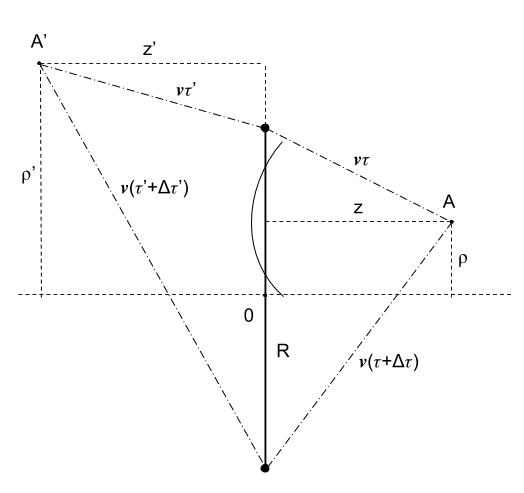
\includegraphics[scale=0.6]{PartialRadiation}
\caption{Фізичний зміст областей випромінювання} \label{fig:part_rad}
\end{center} \end{figure}

Область $ S_2 $ відповідає за події, коли частина кайніх точок джерела вже 
причинно повзязана зі спостерігачем. Тобто частина джерела про яку вже відомо
спостерігачу (часово-поєднані), вже не має круглої форми та ще не охоплює 
всього джерела. В цій області спостерігається деякий перехідний процес в
якому значення прехідної функції поступово згасає на нуль.

Спостервгачі в області $ S_3 $ вже отримали всю інформацію про джерело. Для
них перехідний процес скінчено і зміни напруженності поля не спостерігається,
а отже напруженность електричного поля тут відсутня.

Для зони $ S_3 $ тільки $ E_x $ компонента електричного поля не дорівнює
нулю. Окрім того амплітуда $ E_x $ постійна для всіх подій з облсті $ S_3 $.

Перейдемо до магнітних складових пеехідної функції плаского диску. Для 
отримання магних компонент поля скористаємось еволюційним коефіцієнтом 
\eqref{eq:imh}.

\textcolor{lightgray} { \begin{equation*} \begin{aligned}
\vect{H_\perp} = \frac{1}{\sqrt{\mu_0}} \left( 
\sum \limits_{m=-\infty}^{\infty} \int \limits_{0}^{\infty} d \nu
I_m^h \nabla_\perp \Psi_m + \sum \limits_{n=-\infty}^{\infty}
\int \limits_{0}^{\infty} d \chi I_n^e 
\crossprod{\vect{z_0}}{\nabla_\perp \Phi_n} \right)
\end{aligned} \end{equation*} }
%
\textcolor{lightgray} { \begin{equation*} \begin{aligned}
\nabla_\perp \Psi_m = e^{i m \varphi} \left( \vect{\rho_0} 
\sqrt{\nu} \frac{ J_{m-1}(\nu \rho) - J_{m+1}(\nu \rho) }{2} +
i m \vect{\varphi_0} \frac{J_m(\nu \rho)}{\sqrt{\nu} \rho} \right)
\end{aligned} \end{equation*} }
%
\textcolor{lightgray} { \begin{equation*} \begin{aligned}
\vect{H_\perp} = \frac{1}{\sqrt{\mu_0}} \left( 
\int \limits_{0}^{\infty} d \nu I_{-1}^h \nabla_\perp \Psi_{-1} +
\int \limits_{0}^{\infty} d \nu I_1^h \nabla_\perp \Psi_1 \right) = \\
= - \frac{A_0}{\sqrt{\mu_0}} \int \limits_{0}^{\infty} d \nu
\sqrt{\mu_0} \frac{iR}{4} J_1 (\nu R)
\frac{ U_0 [ W_-, Z ] - U_2 [ W_-, Z ] }{\sqrt{\nu}}  
e^{- i \varphi} \cdot \\ \cdot \left( \vect{\rho_0} 
\sqrt{\nu} \frac{ J_{2}(\nu \rho) - J_{0}(\nu \rho) }{2} +
i \vect{\varphi_0} \frac{J_1(\nu \rho)}{\sqrt{\nu} \rho} \right) -
\frac{A_0}{\sqrt{\mu_0}} \int \limits_{0}^{\infty} d \nu 
\sqrt{\mu_0} \frac{iR}{4} J_1 (\nu R) \cdot \\
\cdot \frac{ U_0 [ W_-, Z ] - U_2 [ W_-, Z ] }{\sqrt{\nu}} 
e^{i \varphi} \left( \vect{\rho_0} 
\sqrt{\nu} \frac{ J_{0}(\nu \rho) - J_{2}(\nu \rho) }{2} +
i \vect{\varphi_0} \frac{J_1(\nu \rho)}{\sqrt{\nu} \rho} \right)
\end{aligned} \end{equation*} }
%
\textcolor{lightgray} { \begin{equation*} \begin{aligned}
H_\varphi = \frac{R A_0}{4} 
\frac{e^{i \varphi} + e^{- i \varphi}}{\rho} \int \limits_{0}^{\infty} 
\frac{d\nu}{\nu} (U_0[ W_-, Z ] - U_2[ W_-, Z ]) J_1(\nu R) J_1(\nu \rho) = \\
= \frac{R}{2} \cos \varphi \int \limits_{0}^{\infty}
\frac{d\nu}{\nu \rho} (U_0[ W_-, Z ] - U_2[ W_-, Z ]) 
J_1(\nu R) J_1(\nu \rho)
\end{aligned} \end{equation*} }
%
\textcolor{lightgray} { \begin{equation*} \begin{aligned}
H_\rho = \frac{R A_0}{4} \frac{e^{i \varphi} - e^{- i \varphi}}{2i}
\int \limits_{0}^{\infty} d \nu (J_{0}(\nu \rho) - J_{2}(\nu \rho))
J_1(\nu R) (U_0[ W_-, Z ] - U_2[ W_-, Z ]) = \\
= \frac{R}{2} \sin \varphi \int \limits_{0}^{\infty} d \nu 
(J_0(\nu \rho) - \frac{J_1(\nu \rho)}{\nu \rho})
J_1(\nu R) (U_0[ W_-, Z ] - U_2[ W_-, Z ]) = \\
\end{aligned} \end{equation*} }
%
\textcolor{lightgray} { \begin{equation*} \begin{aligned}
\vect{H_\perp} \left( r, t \right) = \frac{A_0}{2} \left( 
\vect{\rho_0} \left( I_4 - I_3 \right) \sin \varphi +
\vect{\varphi_0} I_3 \cos \varphi  \right)
\end{aligned} \end{equation*} }
%
\textcolor{lightgray} { \begin{equation*} \begin{aligned}
H_z (r,t) = \frac{1}{\sqrt{\mu_0}} \sum \limits_{m=-\infty}^{\infty}
\int \limits_0^\infty \nu^2 d \nu h_m \Psi_m
\end{aligned} \end{equation*} }
%
\textcolor{lightgray} { \begin{equation*} \begin{aligned}
\Psi_m (\nu) = \frac{J_m(\nu \rho)}{\sqrt{\nu}} e^{im \varphi} 
\end{aligned} \end{equation*} }
%
\textcolor{lightgray} { \begin{equation*} \begin{aligned}
H_z (r,t) = 
\frac{1}{\sqrt{\mu_0}} \int \limits_0^\infty \nu^2 d \nu h_{1} \Psi_{1} +
\frac{1}{\sqrt{\mu_0}} \int \limits_0^\infty \nu^2 d \nu h_{-1} \Psi_{-1}
\end{aligned} \end{equation*} }
%
\textcolor{lightgray} { \begin{equation*} \begin{aligned}
H_z (r,t) = R A_0 \frac{e^{im \varphi}-e^{-im \varphi}}{2} \int_0^\infty 
d \nu J_1(\nu \rho) J_1 (\nu R)
U_1 \left[ -i \nu (ct-z), \nu \sqrt{c^2t^2-z^2} \right]
\end{aligned} \end{equation*} }
%
\textcolor{lightgray} { \begin{equation*} \begin{aligned}
H_z (r,t) = - R A_0 \sin \varphi \int_0^\infty 
d \nu J_1(\nu \rho) J_1 (\nu R) U_1 [ W_-, Z ] = \\
= - i R A_0 \sin \varphi \int_{0}^{\infty} J_1 \left( \nu R \right)
J_1 \left( \nu \rho \right) U_1 [ W_-, Z ]
\end{aligned} \end{equation*} }
%
\textcolor{lightgray} { \begin{equation*} \begin{aligned}
H_z \left( r, t \right) = - A_0 I_5 \sin \varphi
\end{aligned} \end{equation*} }
%
\begin{equation} \label{eq:linear_h_cyl}
\vect{H} (r, t) = \frac{A_0}{2} \Big( 
\vect{\rho_0} \left( I_4 - I_3 \right) \sin \varphi +
\vect{\varphi_0} I_3 \cos \varphi -
2 \vect{z_0} I_5 \sin \varphi \Big),
\end{equation}
%
де 
%
\begin{equation*}
I_3 = R \int \limits_{0}^{\infty}
\frac{d\nu}{\nu \rho} J_1(\nu R) J_1(\nu \rho)
\Big( U_0[ W, Z ] - U_2[ W, Z ] \Big),
\end{equation*}
%
\begin{equation*}
I_4 = R \int \limits_{0}^{\infty} d\nu J_1(\nu R) J_0(\nu \rho)
\Big( U_0[ W, Z ] - U_2[ W, Z ] \Big),
\end{equation*}
%
\begin{equation*}
I_5 = i R \int \limits_0^\infty 
d \nu J_1(\nu \rho) J_1 (\nu R)
U_1 \left[ -i \nu \left( \frac{ct}{\sqrt{\epsilon \mu}} - z \right), 
\nu \sqrt{\frac{c^2t^2}{\epsilon \mu}-z^2} \right].
\end{equation*}

В Декартовому базисі вектор напруженності магнітного поля матиме вигляяд

\begin{equation} \begin{aligned} \label{eq:Hxyz}
\left( \begin{array}{c} H_x \\ H_y \\ H_z \end{array} \right) = 
\frac{A_0}{2} \sqrt{\frac{\mu_0 \mu}{\epsilon_0 \epsilon}} 
\left( \begin{array}{c}
- I_4 \sin \varphi \cos \varphi \\
I_3 \cos^2 \varphi + (I_4 - I_3) \sin^2 \varphi \\
- 2 I_5 sin \varphi
\end{array} \right).
\end{aligned} \end{equation}

Для інтегралів $ I_3, I_4, I_5 $ аналітичні розв'язки, які представлено в 
додатку \ref{ch:lommel}, вдалось знайти лише на осі випромінювання 
($ \rho = 0 $). Відзначимо, що всі інтеграли мають дійсні значення, що витікає
з властивостей функції Ломмеля. Застсовуючи визначення функції Ломеля для  
виразу \eqref{eq:linear_h_cyl} на великій відстані від джерела, де плаский 
диск можна розгядати, як матеріальну точку, тобто $ z >> R $ помічаємо, що 
%
\begin{equation*}
U_0[ W, Z ] - U_2[ W, Z ] = 
J_0 \left( \frac{c^2t^2}{\epsilon \mu}  - z^2 \right),
\end{equation*}
%
тоді ортогональні поперечні компоненти електромагнітного поля попарно 
пропорційні через значення імпедансу вільного простору, в якому 
розповлюджується хвиля
%
\begin{equation} \label{eq:e2h}
\frac{E_x}{H_y} = \frac{E_y}{H_x} = 
\sqrt{\frac{\mu_0 \mu}{\epsilon_0 \epsilon}},
\end{equation}
%
що відповідає властивостям пласної хвилі, а також підтверждує можливість 
апроксимації антен імпульснго випромінювання фізичною моделю плаского 
сторонього електричного струму. Такий висновку можна дійти з того, що
саме пласку хвилю очікується побачити після випрямлення сфкричного фонту
від ТЕМ рупора в плаский гіперболічною, або витягноную сферичною лінзою.

Звертаючись до аналітики з додатку \ref{ch:lommel} також помічаємо, що 
рівність \eqref{eq:e2h} також строго виконується і вблизу апертури, для 
всієї тривалості перехідного процесу. Рівність не виконується лише для 
області $ S_3 $, де $ \vect{E} = 0 $, а $ \vect{H}_\perp = const $.

%%%%%%%%%%%%%%%%%%%%%%%%%%%%%%%%%%%%%%%%%%%%%%%%%%%%%%%%%%%%%%%%%%%%%%%%%%%%%%%
\section{Властивості перехідної функції плаского диску}

\begin{figure}[h] \begin{center}
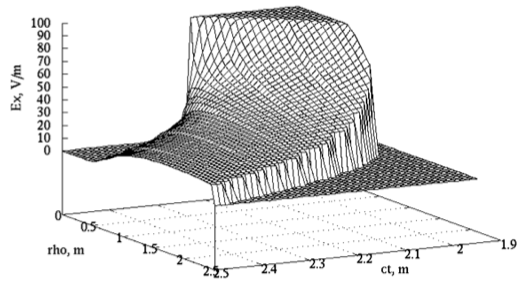
\includegraphics[scale=1.6]{MissileEffect}
\caption{Ефект електромагнітного снаряду ($ z = 2 $ м)} \label{fig:emp_rho}
\end{center} \end{figure}
%
\begin{figure}[h] \begin{center}
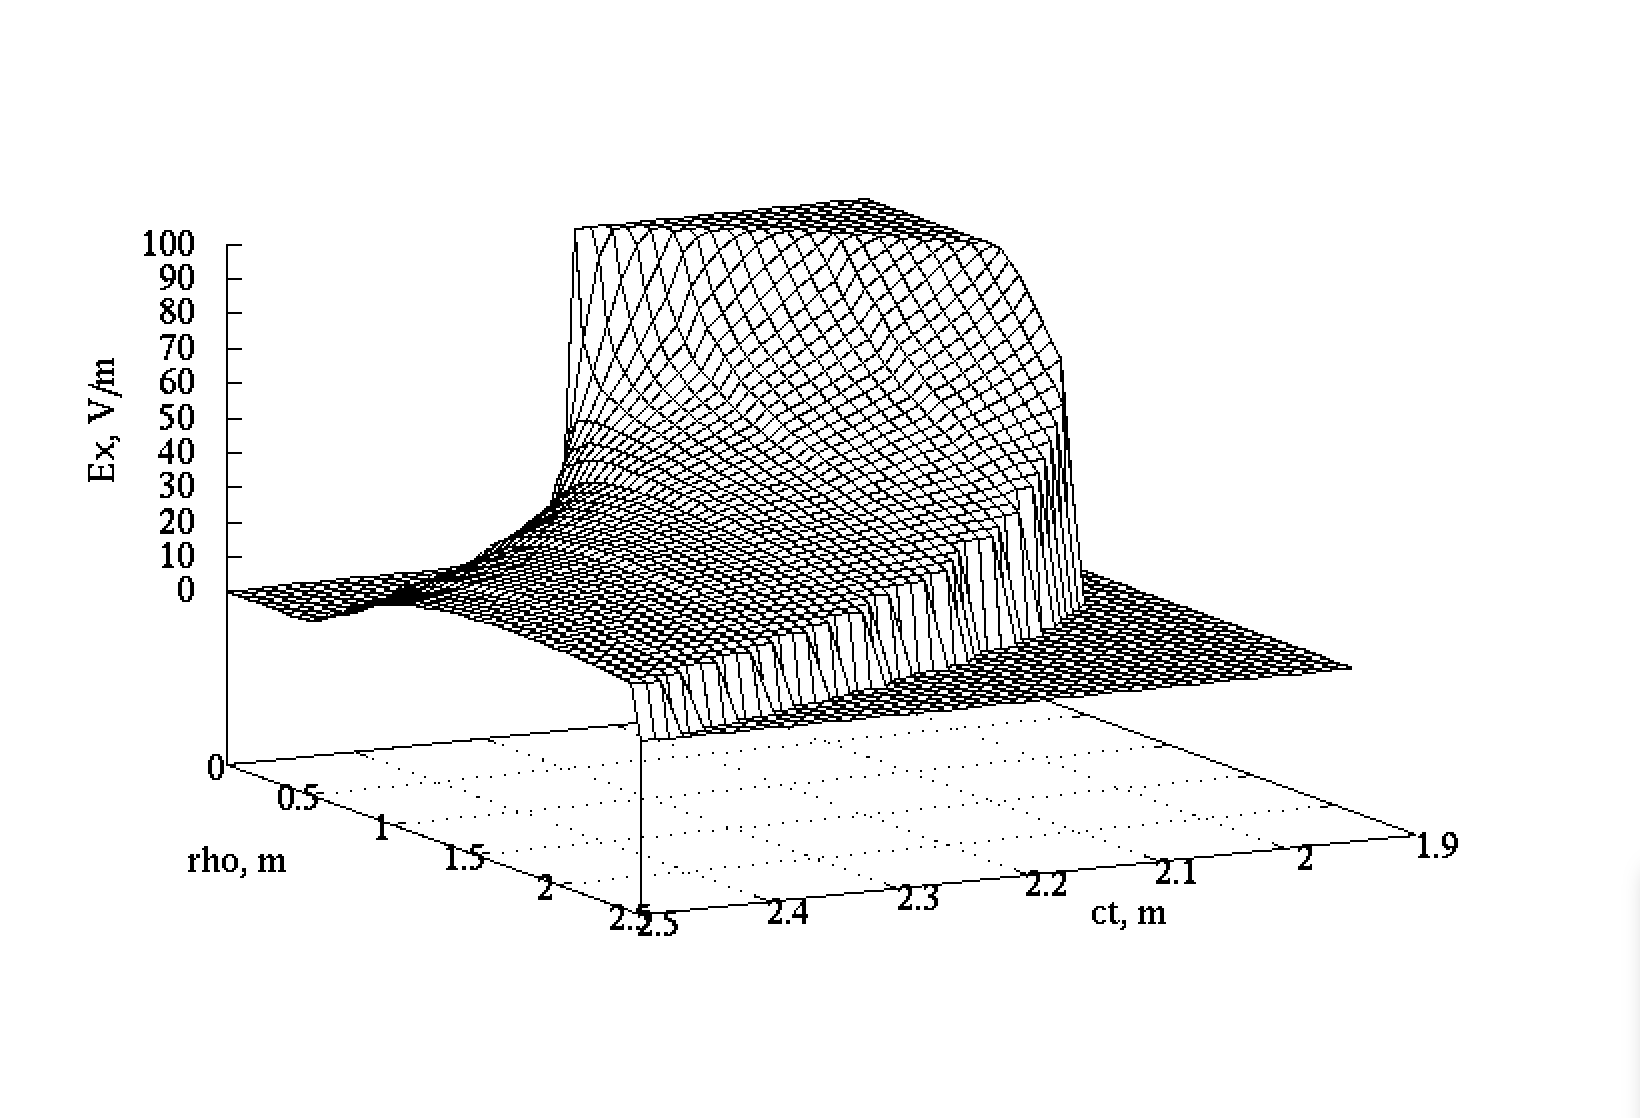
\includegraphics[scale=0.6]{TransientEffect}
\caption{Ефект електромагнітного снаряду ($ \rho = 0.2 $ м)} \label{fig:emp_z}
\end{center} \end{figure}
%
\begin{figure}[h] \begin{center}
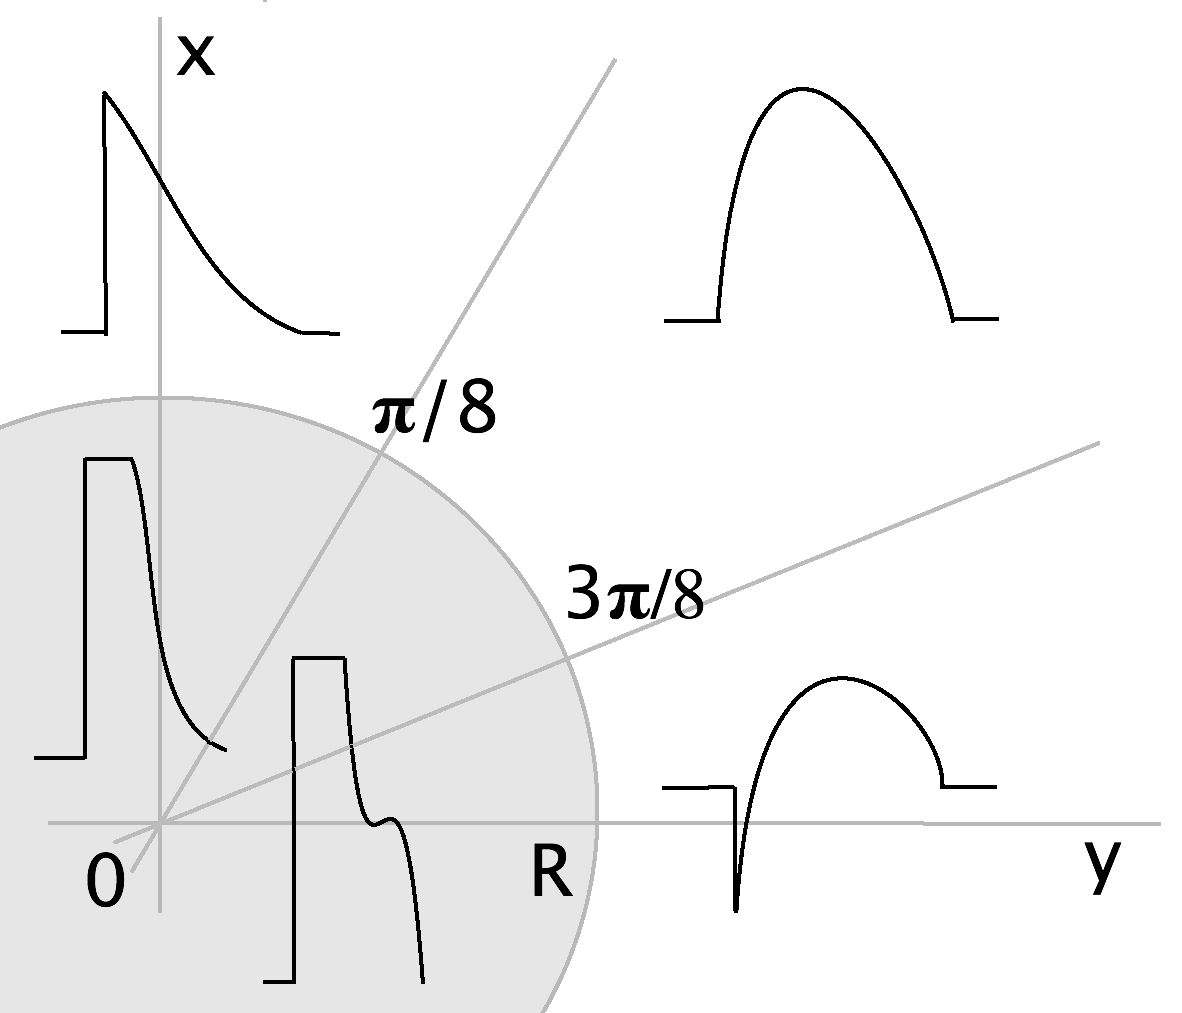
\includegraphics[scale=0.7]{LinearPulsShape}
\caption{Кутова залежнысть формы імпульсу ($ \rho = R/2 .. 2R $ м)} 
\label{fig:emp_shape}
\end{center} \end{figure}
%
\begin{figure}[h] \begin{center}
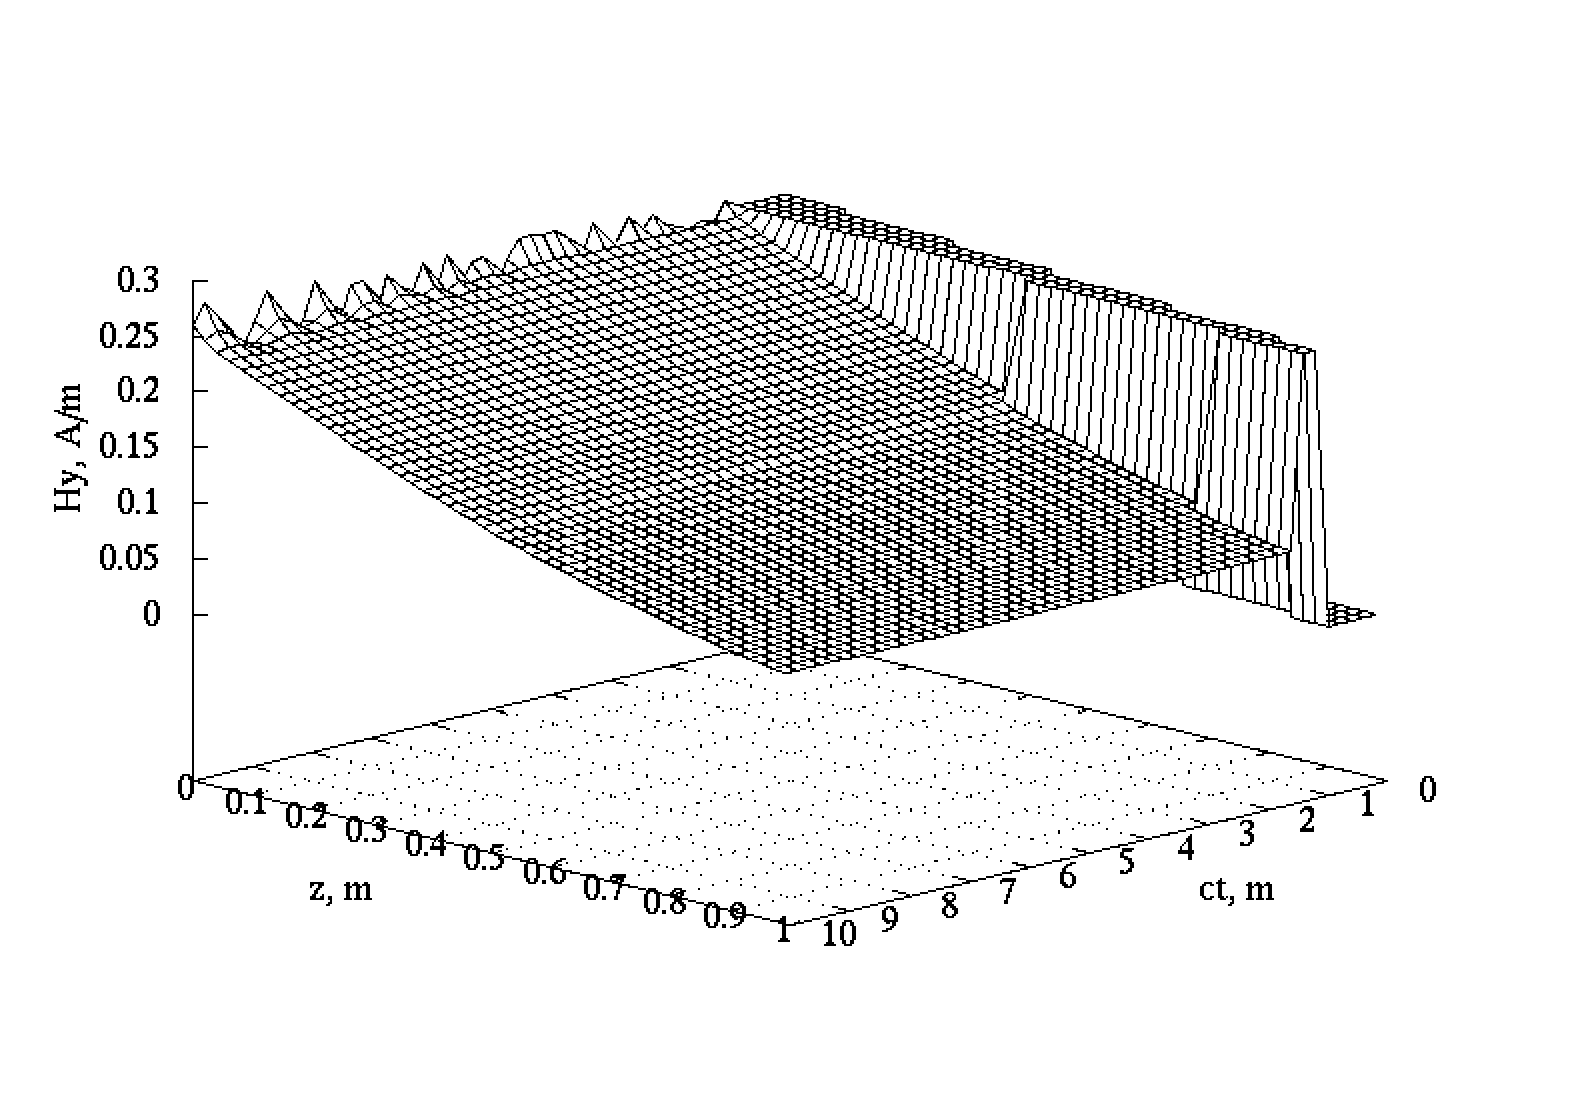
\includegraphics[scale=0.6]{StaticOnAxis}
\caption{Магнітно-статичне поле ($ \rho = 0 $ м)} \label{fig:emp_h_rho}
\end{center} \end{figure}
%
\begin{figure}[h] \begin{center}
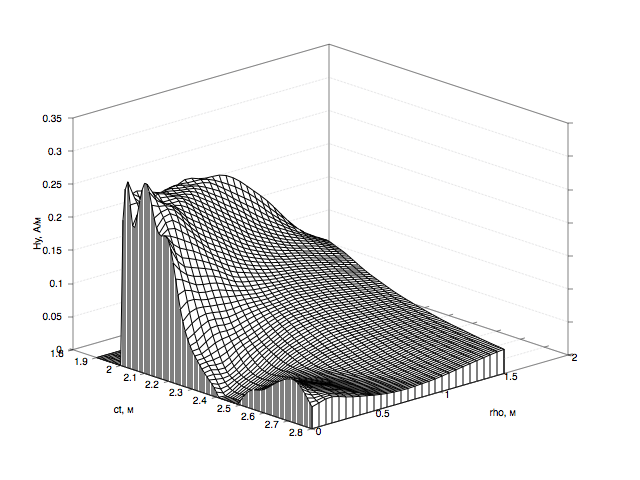
\includegraphics[scale=0.7]{LinearMagnetic}
\caption{Магнітно-статичне поле ($ z = 2 $ м)} \label{fig:emp_h_rho}
\end{center} \end{figure}
%
\begin{figure}[h] \begin{center}
\includegraphics[scale=0.9]{Ex_vs_Hz}
\caption{$E_x$ і $H_z$ в ($\rho = R/2$, $\varphi = -\pi/2$, $z = R$)} 
\label{fig:ex_vs_hz}
\end{center} \end{figure}

Область електромагнітного знаряду $ S_1 $ характерезується сталою амплітудою 
електричного і мігнітного поля в кожен момент часу. Також в цій області 
існують лише дві кмпоненти поля $ E_x $ та $ H_y $, що видно з аналітики в 
додатках \ref{ch:bessel} та \ref{ch:lommel}, а отже в області 
електромгнітного знаряду спостерігається вироджена ТЕМ хвиля. Спостерігач на 
осі випромінювання знаходиться в області елктромагнітного знаряду вподовж 
всього перехідного процесу, бо стає \textcolor{red}{часовоподібним} відносно 
всіх крайніх точок джерела одномоментно. Таким чином для $ \rho = 0 $ область 
визначення векотрів \eqref{eq:Exyz} та \eqref{eq:Hxyz} завжди $ S_1 $, отже
значення сталих амплітуд поля в області електромагнітного знаряду знайдемо
підставивши $ \rho = 0 $ в \eqref{eq:Exyz} та \eqref{eq:Hxyz}:

\begin{equation*} \begin{aligned}
\vect{E} \{ S_1 \} = 
\vect{x_0} \frac{A_0}{4} 
\sqrt{\frac{\mu_0 \mu}{\epsilon_0 \epsilon}};
\end{aligned} \end{equation*}
%
\begin{equation*} \begin{aligned}
\vect{H} \{ S_1 \} = \vect{y_0} \frac{A_0}{4}.
\end{aligned} \end{equation*}
%

Співвідносячи форму імпульсу ра Рис.~\ref{fig:emp_rho} з тим, що 
$ H_z \{ S_1 \} = 0 $ бачимо, що поперечне електромагнітне поле в бласті 
$ S_1 $ "випереджує" поздовжне та ніби породжує його в області $ S_2 $. В 
роботах Фарадея зустрічається твердження, що випромінює не антена а простір 
довкола неї. Саме це і спостерігається в області електромагнітного знаряду - 
поздовжна компонента поля, без якої неможливе розповсюдження хвилі у 
вільному просторі \textcolor{red}{[Хармут]}, породжується простором у 
якому з’являється поперечні компоненти. Таким чином, можимо узагальнити 
твеждженн Хармута для нестаціонарного процесу: розповсюдження хвилі, а тобто 
($ E_z \neq 0 $ чи $ H_z \neq 0 $) почнется тільки тоді, коли спостерігач 
дізнається про те, що розподіл заряду стороннього джерела змінюєтья у часі 
або у просторі, а до цього, хвиля не розповсюджується, не дивлячись на те, 
що спостерігач і джерело - вже причино пов'язані. 

Можемо зробити висновок, що для стаціонарного процесу поняття поля и хвилі 
тотожні, коли у часовій області інколи ні: так наприклад область визначеня 
електрично поля, що випромінюеться пласким диском $ S_1 S_2 S_3 $, а для 
область визначення хвилі лише $ S_2 S_3 $, тобто електромагнітний сназяд 
неможна назвити хвилею, а лише полем.

%
Такий ефект носить назву електромагнітного знаряду. Хоча поле в явному
виді не залежить від точки спостереження, залежність присутня в визначенні 
зон випромінювання поля плаского диску. Користуючить ними можна вирахувати 
тривалість ефекту.
%
\begin{equation*} \begin{aligned}
\frac{c \tau}{\sqrt{\epsilon \mu}} = \sqrt{R^2+z^2} - z.
\end{aligned} \end{equation*}
%
При $ R = 1 $ можна ввести апроксимацію цієї формули, як  
%
\begin{equation*} \begin{aligned}
\frac{c \tau}{\sqrt{\epsilon \mu}} \left( z \gg 2R \right) \approx 
\begin{cases}
\frac{2R}{z} , R \geq 1 \\
\frac{R^2}{2z} , R \leq 1
\end{cases}
\end{aligned} \end{equation*}


За визначенням дальньої зони - це область простору, де $ E_\varphi = H_\rho $ та
$ H_\varphi = E_\rho $. Дня лінійного поля плаского диску ці умови виконується, 
коли $ U_0(W_-,Z) - U_2(W_-,Z) = J_0(Z) $. Остання тотожність математично вірна
тоді і тільки коли 
%
\begin{equation} \label{eq:FraunhoferDistance}
\left. \lim_{z \to \infty} \left( \frac{ct-z}{ct+z} \right)^m 
\right|_{m > 1} = 0
\end{equation}
%
Остання тотожність є умовою дальньої зони для антени що породжує 
нестаціонарне поле. Варто зазначити, що при рості $ z $ росте і $ t $, 
відповідно до принципу причинності, тобто умова $ ct - z > 0 $ виконується.
%
\begin{figure}[h] \begin{center}
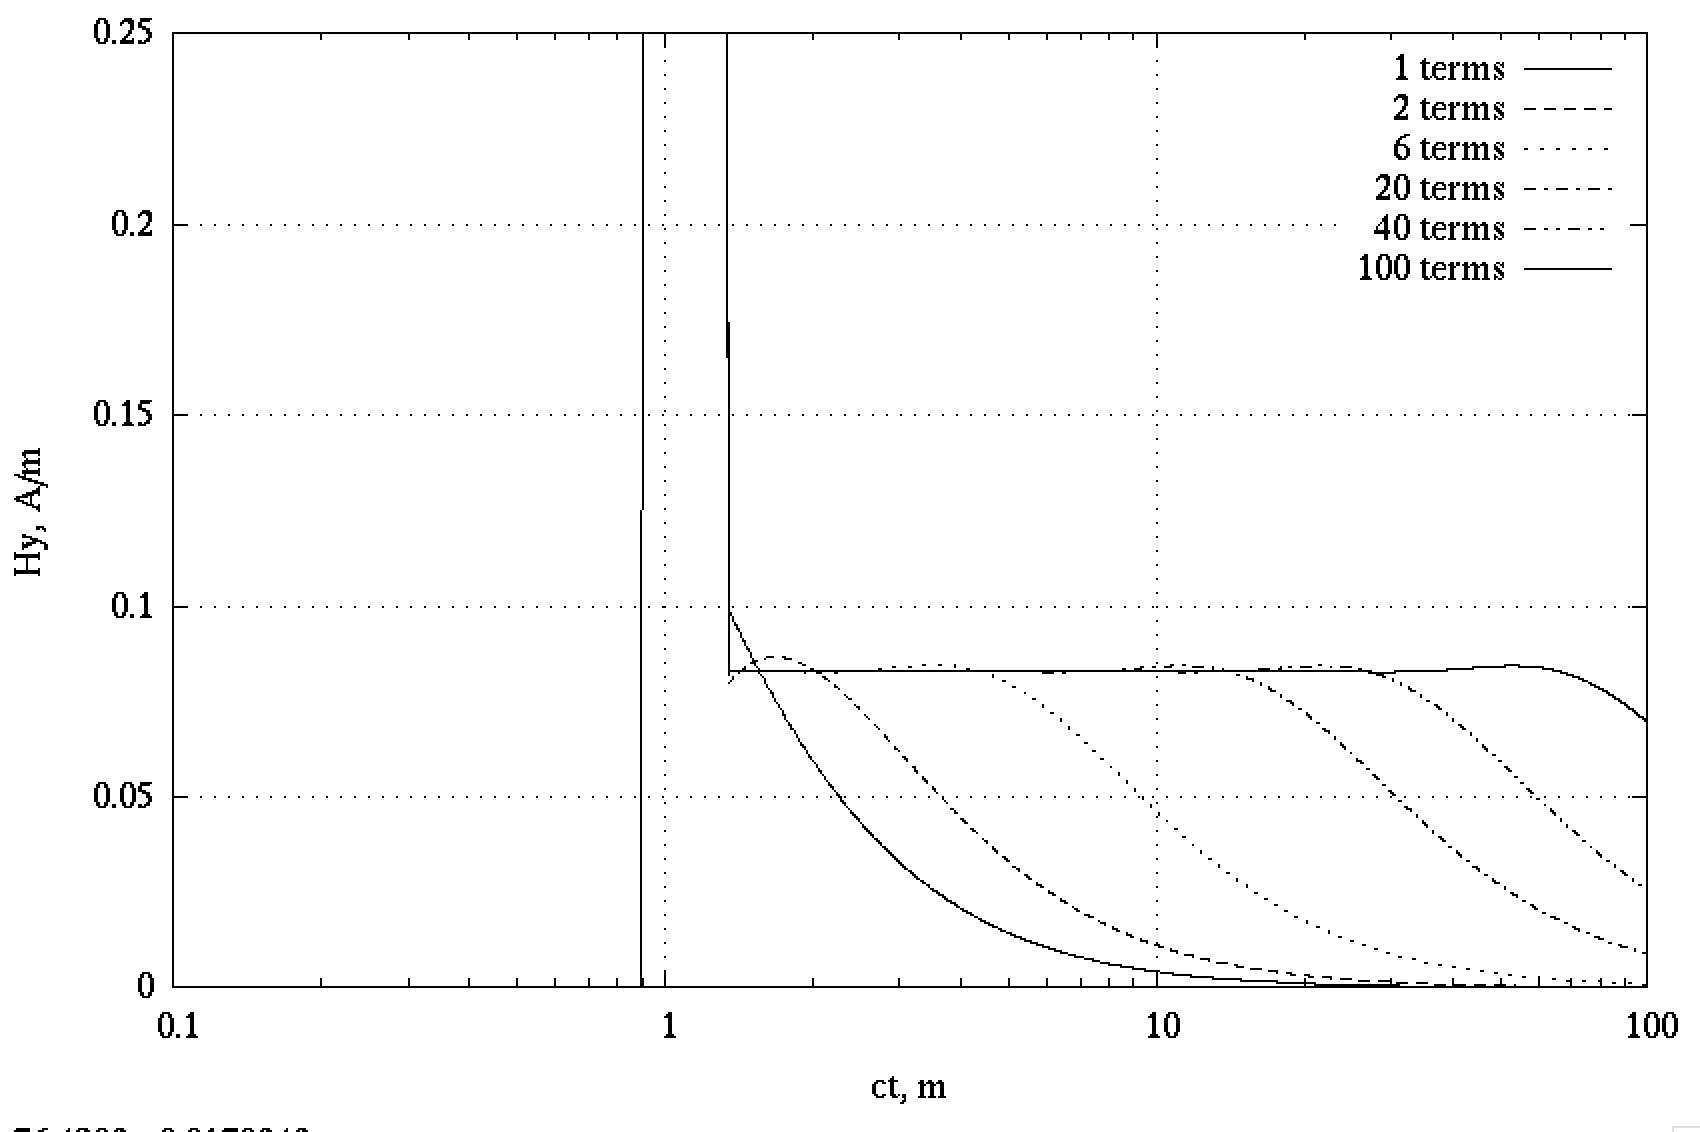
\includegraphics[scale=0.5]{SingulatiyFactorization}
\caption{Розклад сингулярності джерела} \label{fig:singulatiy_factorization}
\end{center} \end{figure}
%
Побудуємо діаграму спрямованності випроміювача корістуючись різницею 
максимального та мінімального значення електричного поля, збудженого 
випромінюванням перехідної функції, як функцію азимутального кута в площінах. 

\textcolor{red} { Плаский диск можна розглядати, як генератор пласної хвилі,
тоді антенни Баума та Ву можна розглядати, як генератори квазі-пласкої хвилі }

%%%%%%%%%%%%%%%%%%%%%%%%%%%%%%%%%%%%%%%%%%%%%%%%%%%%%%%%%%%%%%%%%%%%%%%%%%%%%%
\section{Збуджуючий імпульс довільної форми}

Узагальнюючи принцип суперпозиції...

Користуючитсь інтегралом Дюамеля \cite[ст. 40]{imp:Kharkevich1950} можно 
отримати випромінювання...
%
\begin{equation}
\vect{E} = \int_{0}^{t} f(\tau) \vect{E_0} (t - \tau) d \tau,
\end{equation}
%
де $ \vect{E_0} $ - імпльсна характеристика антенни, а $ f(\tau) $ - 
плавна функція часу довільного виду. Користуючись переставною властивістью 
інтегралу цю формулу
%
Чим більше кінець відгуку схожий на початок тим ближче точка спостереження
до осі випромінювання. Це справедливо для будьякої антенни та довільної форми
імпульсу.

%%%%%%%%%%%%%%%%%%%%%%%%%%%%%%%%%%%%%%%%%%%%%%%%%%%%%%%%%%%%%%%%%%%%%%%%%%%%%%
\section{Енергія імпульсного випромінювання}

Побудова класичної енергетичної діаграми спрямованості мало інформативна 
для імпульсного випромінювання. Будуватимемо поперечні зрізи значень енергій
для різних довжин імпульсів та для різних відстаней від джерела.
Для збереженя кутового розміру зрізів візьмемо йщго $ z + 2 \cdot R $.
%
\begin{equation}
W = \int_{0}^{\infty} \vect{E}^2 (t) dt
\end{equation}
%
\textcolor{lightgray} { \begin{equation}
W = \int_{0}^{\infty} \left( E_\rho^2 + E_\varphi^2 + E_z^2 \right) dt
\end{equation} }
%
Якщо відомо час приходу імпульсу в точку спостереження та його тривалість, 
можна обмежити область інтегрування.
%
\begin{equation}
W = \int_{\tau_1}^{\tau_2} \left( E_\rho^2 + E_\varphi^2 + E_z^2 \right) dt
\end{equation}
%
\textcolor{lightgray} { \begin{equation*}
(\rho-R)^2 > v^2t^2 - z^2
\end{equation*} }
%
\textcolor{lightgray} { \begin{equation*}
v^2t^2 = (\rho-R)^2 + z^2
\end{equation*} }
%
\textcolor{lightgray} { \begin{equation*}
vt = \sqrt{(\rho-R)^2 + z^2}
\end{equation*} }
%
\begin{equation*}
\tau_1 = \sqrt{(\rho-R)^2 + z^2}
\end{equation*}
%
\begin{equation*}
\tau_2 = \tau + \sqrt{(\rho-R)^2 + z^2}
\end{equation*}
%
Для зручності застосування формули домножимо ліву і праву частину на
швидкість світла в середовищі $ v $ та згадаємо, що $ E_z = 0 $.
%
\begin{equation}
v W(r) = \int_{\tau_1}^{\tau_2} 
\Big( E_\rho^2 (vt,r) + E_\varphi^2 (vt,r) \Big) dvt
\end{equation}
